\begin{center}
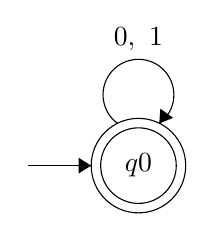
\begin{tikzpicture}[scale=0.2]
\tikzstyle{every node}+=[inner sep=0pt]
\draw [black] (21.3,-32) circle (3);
\draw (21.3,-32) node {$q0$};
\draw [black] (21.3,-32) circle (2.4);
\draw [black] (14.3,-32) -- (18.3,-32);
\fill [black] (18.3,-32) -- (17.5,-31.5) -- (17.5,-32.5);
\draw [black] (19.977,-29.32) arc (234:-54:2.25);
\draw (21.3,-24.75) node [above] {$0,\mbox{ }1$};
\fill [black] (22.62,-29.32) -- (23.5,-28.97) -- (22.69,-28.38);
\end{tikzpicture}
\end{center}
